
% Q15
\question In the figure, the volume of the solid right triangular prism is

\begin{minipage}{0.45\textwidth}
\begin{choices}
    \choice $544\text{ cm}^3$ .
    \choice $600\text{ cm}^3$ .
    \choice $660\text{ cm}^3$ .
    \correctchoice $720\text{ cm}^3$ .
\end{choices}
\end{minipage}
\begin{minipage}{0.52\textwidth}
\centering
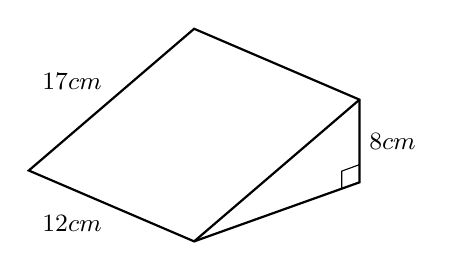
\begin{tikzpicture}[scale=0.75]
    \coordinate (A) at (0,1.2);
    \coordinate (B) at (2.8,0);
    \coordinate (C) at (5.6,1.0);
    \coordinate (D) at (5.6,2.4);
    \coordinate (E) at (2.8,3.6);
    \draw[thick] (A) -- (B) -- (C) -- (D) -- (E) -- cycle;
    \draw[thick] (B) -- (D);
    \draw (5.3,0.89) -- (5.3,1.19) -- (5.6,1.3);
    \node[above left] at (1.4,2.4) {\small $17\text{ cm}$};
    \node[below left] at (1.4,0.6) {\small $12\text{ cm}$};
    \node[right] at (5.6,1.7) {\small $8\text{ cm}$};
\end{tikzpicture}
\end{minipage}
\begin{solution}
The base of the right-angled triangle is $\sqrt{17^2 - 8^2} = 15\text{ cm}$. \\
Volume of the prism $= \frac{1}{2}(15)(8)(12) = 720\text{ cm}^3$ (D).
\end{solution}

% Q16
\question In the figure, $ABCD$ is a parallelogram. $E$ is a point lying on $BC$ such that $BE : EC = 5 : 3$ . $AE$ and $BD$ intersect at the point $F$ . If the area of $\triangle ABF$ is $120\text{ cm}^2$ , then the area of the quadrilateral $CDFE$ is

\begin{minipage}{0.45\textwidth}
\begin{choices}
    \correctchoice $237\text{ cm}^2$ .
    \choice $307\text{ cm}^2$ .
    \choice $312\text{ cm}^2$ .
    \choice $429\text{ cm}^2$ .
\end{choices}
\end{minipage}
\begin{minipage}{0.52\textwidth}
\centering
\begin{tikzpicture}[scale=0.8]
    \coordinate (B) at (0,0);
    \coordinate (C) at (4.8,0);
    \coordinate (A) at (1.4,3.2);
    \coordinate (D) at (6.2,3.2);
    \coordinate (E) at (3.0,0);
    \path[name path=AE] (A) -- (E);
    \path[name path=BD] (B) -- (D);
    \path[name intersections={of=AE and BD, by=F}];
    \draw[thick] (A) -- (B) -- (C) -- (D) -- cycle;
    \draw[thick] (A) -- (E);
    \draw[thick] (B) -- (D);
    \node[above left] at (A) {$A$};
    \node[below left] at (B) {$B$};
    \node[below right] at (C) {$C$};
    \node[above right] at (D) {$D$};
    \node[below] at (E) {$E$};
    \node[above=10pt, right=-5pt] at (F) {$F$};
\end{tikzpicture}
\end{minipage}
\begin{solution}
Since $\triangle BFE \sim \triangle DFA$ and $BE : DA = 5 : 8$, we have $EF : FA = BF : FD = 5 : 8$. \\
Thus $\text{Area}(\triangle BFE) = \frac{5}{8}(120) = 75\text{ cm}^2$ and $\text{Area}(\triangle DFA) = \frac{8}{5}(120) = 192\text{ cm}^2$. \\
Then $\text{Area}(\triangle BCD) = \text{Area}(\triangle ABD) = 120 + 192 = 312\text{ cm}^2$. \\
Therefore, $\text{Area}(CDFE) = 312 - 75 = 237\text{ cm}^2$ (A).
\end{solution}

% Q17
\question In the figure, $O$ is the centre of the sector $OABCD$ . $AD$ and $OC$ are perpendicular to each other and intersect at the point $E$ . $F$ is a point lying on $AD$ such that $BF$ is perpendicular to $AD$ . If $AF = 9\text{ cm}$ , $DF = 39\text{ cm}$ and $OE = 18\text{ cm}$ , then the area of the sector $OBC$ is

\begin{minipage}{0.45\textwidth}
\begin{choices}
    \choice $48\pi\text{ cm}^2$ .
    \correctchoice $75\pi\text{ cm}^2$ .
    \choice $96\pi\text{ cm}^2$ .
    \choice $150\pi\text{ cm}^2$ .
\end{choices}
\end{minipage}
\begin{minipage}{0.52\textwidth}
\centering
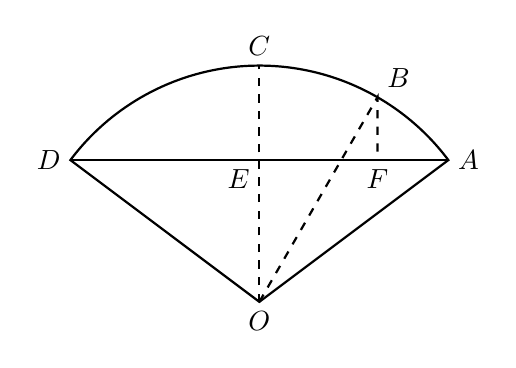
\begin{tikzpicture}[scale=0.1]
    \def\R{30}
    \coordinate (O) at (0,0);
    \coordinate (C) at (0,\R);
    \coordinate (E) at (0,18);
    \coordinate (D) at (-24,18);
    \coordinate (A) at (24,18);
    \coordinate (F) at (15,18);
    \coordinate (B) at (15,25.98);
    \draw[thick] (O) -- (A) arc (36.87:143.13:\R) -- cycle;
    \draw[thick] (D) -- (A);
    \draw[thick,dashed] (O) -- (C);
    \draw[thick,dashed] (O) -- (B) -- (F);
    \node[below] at (O) {$O$};
    \node[right] at (A) {$A$};
    \node[above right] at (B) {$B$};
    \node[above] at (C) {$C$};
    \node[left] at (D) {$D$};
    \node[below left] at (E) {$E$};
    \node[below] at (F) {$F$};
\end{tikzpicture}
\end{minipage}
\begin{solution}
Since $OC \perp AD$, $E$ is the mid-point of $AD$, so $AE = \frac{9+39}{2} = 24\text{ cm}$ and $EF = 24 - 9 = 15\text{ cm}$. \\
In right-angled $\triangle OEA$, the radius is $OA = OB = \sqrt{18^2 + 24^2} = 30\text{ cm}$. \\
Since the perpendicular distance from $B$ to $OC$ is $EF = 15\text{ cm}$, we have $\sin\angle BOC = \dfrac{15}{30} = \dfrac{1}{2} \implies \angle BOC = 30^\circ$. \\
Area of sector $OBC = \pi(30)^2 \times \dfrac{30^\circ}{360^\circ} = 75\pi\text{ cm}^2$ (B).
\end{solution}